\data{06/11/2019}
\chapter{Evaluation}
\section{Introduction}
Evaluation requires to define one or more measure which have to be optimized. For such reason, they need to be quantitative. \newline
In principle, when training a model we'd like to know its performance on the entire domain where it's going to be applied, but this is not possible due to the generalization error\footnote{Since learning algorithms are evaluated on finite samples, the evaluation of a learning algorithm may be sensitive to sampling error, i.e., measurements of prediction error on the current data may not provide much information about predictive ability on new data.}, hence an approximation is needed.\newline
Performance evaluation is needed for:
\begin{itemize}
  \item Tuning hyperparameters\footnote{All those parameters that are not learned, but are set at the beginning by the programmer, e.g. the type of kernel and parameters or the learning rate of a perceptron.} of learning method;
  \item Evaluating quality of learned predictor;
  \item Computing statistical significance of difference between learning algorithms.
\end{itemize}
Notice that we cannot evaluate on the training set since, if were to do so, we would end up with overfitting. \newline
Mind that hyperparameters can be machine learned by trying different possibilities and automatically choosing the best one. \newline
When we talked about parameters estimation, we talked about, e.g., maximum likelihood and maximum a posteriori. This functions allows to learn good values for the weights. In supervised learning, a machine learning algorithm builds a model by examining many examples and attempting to find a model that minimizes loss; this process is called \textit{empirical risk minimization}. \textbf{Loss} is the penalty for a bad prediction, that is, loss is a number indicating how bad the model's prediction was on a single example: if the model's prediction is perfect, then loss is zero, otherwise is grater. The goal of training a model is to find a set of weights that have low loss, on average, across all examples.  \newline
In general we can say that the training loss function measures the cost paid for predicting $f(\vect{x})$ for output $y$. \newline
Notice that training loss and performance measure are two different things, the first one is used in training, the second is used to evaluate the performance of the model. \newline
Multiple performance measures could be used to evaluate different aspects of a learner. 
%
%
%
\section{Binary classification -- Confusion Matrix}
In order to evaluate binary classification, one could use a confusion matrix, that is a matrix that reports the true labels (on rows) and the predicted labels (on columns). Each cell tells how many value have been predicted correctly, and if not what was the mistake. \newline
Each can belong to one of the following cases:
\begin{itemize}
  \item True positives: positives that were predicted positive;
  \item True negatives: negatives that were predicted negative;
  \item False positives: negatives that were predicted positive;
  \item False negatives: positives that were predicted negative.
\end{itemize}
\begin{center}
  \begin{tabular}{c|c|c}
    \diagbox[width=10em]{True}{Pred} &Positive       &Negative\\
    \hline
    Positive              &True Positive  &False Negative\\
    \hline
    Negative              &False Positive &True Negative
  \end{tabular}
\end{center}
This matrix is useful because ti gives a picture of what the predictor does. For example consider the following table:
\begin{center}
	\begin{tabular}{ccc}
	\diagbox[width=10em]{True}{Pred}& Pos&Neg\\
	Pos& 0 &10\\
	Neg& 0 &90
	\end{tabular}
\end{center}
It's possible to see that the predictor is biased in not predicting any positive: 1 out of 10 samples where predicted false but actually were positive, hence they were false negatives. \newline
Over the confusion matrix we can compute the following metrics:
\begin{itemize}
  \item \textbf{Accuracy}: it says how many samples were predicted correctly. 
  \item \textbf{Precision}: it says how accurate the model is when predicting positive;
  \item \textbf{Recall} or \textbf{sensitivity}: how many positive example we got with respective to the true positive.
  \item \textbf{Aggregate measures}: for instance, \textit{F-Measure} that combines precision and recall.
\end{itemize}
%
%
\subsection{Accuracy}
Accuracy is the fraction of correctly labelled examples among all predictors. 
\[Acc=\frac{TP+TN}{TP+TN+FP+FN}\]
It's a scoring function, so the bigger the value the better. Notice that the accuracy is actually one minus the misclassification cost. \newline
Two bigger problems are bound to the accuracy:
\begin{itemize}
  \item It cannot be used for training;
  \item In strongly unbalanced datasets (typically when negatives are much more than positives) it is not informative: predictions are dominated by the larger class. Considering the example before, the accuracy was $0.9$, but looking at all the table it's possible to see how it learned only to predict negatives. It's possible to rebalance the costs, e.g. a single positive counts as $\myfrac{N}{P}$ where $N=TN+FP$ and $P=TP+FN$.
\end{itemize}
This cannot be used for training, its also problematic as an evaluation metric as some datasets are too unbalanced as the table before. The accuracy of the previous was 0.9, but this has learned only to predict negatives. If we hadn't looked at the confusion matrix we wouldn't have noticed. 
%
%
\subsection{Precision}
Precision is the fraction of positives among examples predicted as positives, so it measures the precision of a learner when predicting positive. 
\[Pre=\frac{TP}{TP+FP}\]
%
%
\subsection{Recall}
It is the fraction of positive examples predicted as positives, so it measures the coverage of the learner in returning positive examples.
\[Rec=\frac{TP}{TP+FN}\]
    the complement of precision:  This two measures are contradictory: if we want to be really precise we'll predict positive less frequently and so recall will be lower.
%
%
\subsection{Aggregate Metrics -- F-Measure}
Precision and recall are complementary, so increasing the precision typically reduces the recall. F-measure combines the two measures balancing the two aspects:
\[F_\beta=\frac{(1+\beta^2)(Pre\times Rec)}{\beta^2Pre+Rec}\]
$\beta$ is the parameter that trades-off precision and recall.
%
\subsubsection{$F_1$}
If $\beta=1$, we have $F_1$-measure. This is actually the harmonic mean of precision and recall:
\[F_1=\frac{2(Pre\times Rec)}{Pre+Rec}\]
%
%
\subsection{Precision-Recall Curve}
Classifiers often provide a confidence in the prediction. A hard decision is made setting a threshold on the classifier. When we compute one of the above measures, we are actually computing it for a specific threshold. It is possible to change the threshold if interested in maximizing a specific performance, e.g. recall. \newline
We can do so by plotting a graph representing the values for each threshold:
\begin{center}
  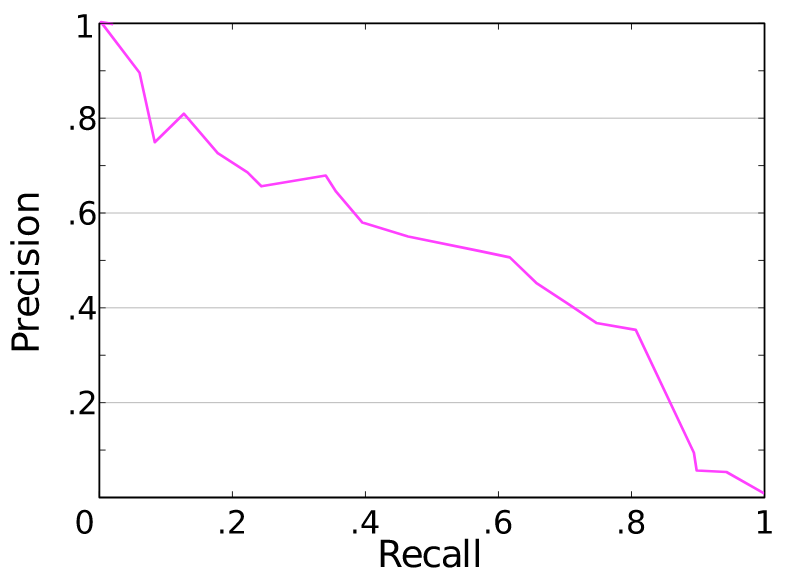
\includegraphics[width=0.6\linewidth]{PrecisionRecallCurve}
\end{center}
It is possible to investigate the performance of the learner in different scenarios. \newline
A single aggregate value can be obtained by taking the area under the curve. A high value means both high precision and recall, while a lower value doesn't give information regarding each one of the measures.
\begin{center}
  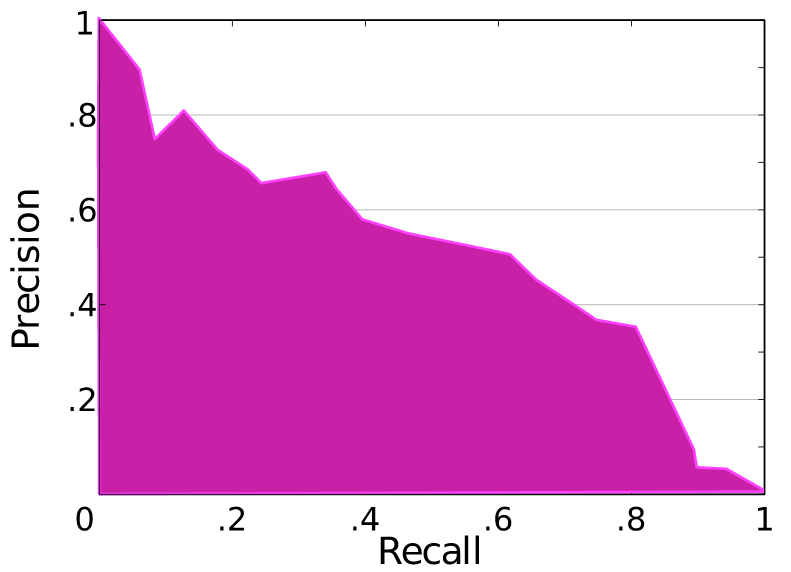
\includegraphics[width=0.6\linewidth]{PrecisionRecallArea}
\end{center}
Notice that when recall is 0 also precision is 0, and vice versa, so we have a discontinuity. 
%
%
%
\section{Multiclass Classification}
Binary matrix can be extent to multi-class. \newline
\begin{center}
  \begin{tabular}{r|c|c|c}
    \diagbox[width=10em]{True}{Pred}&$y_1$    &$\hdots$ &$y_M$\\
    \hline
    $y_1$                           &$n_{11}$ &$\hdots$ &$n_{1M}$\\
    \hline
                                    &$\vdots$ &$\vdots$ &$\vdots$\\
    \hline
    $y_M$                           &$n_{M1}$ &$\hdots$ &$n_{MM}$
  \end{tabular}
\end{center}
$n_{ij}$ is the number of examples with class $y_i$ predicted as $y_j$. \newline
The main diagonal contains the true positives for each class, while false positives $FP_i$ are given by the sum of off-diagonal elements along a column and false negatives $FN_i$ are given by the sum of off-diagonal elements along a row:
\[FP_i=\Sum_{j\neq i}n_{ji}\qquad FN_i=\Sum_{j\neq i}n_{ij}\]
Even the metrics are computed per class, for example:
\[Pre_i=\frac{n_{ij}}{n_{ij}+FP_i}\qquad Rec_i=\frac{n_{ij}}{n_{ij}+FN_i}\]
There is then a global metric that's called \textit{multiclass accuracy} that is the sum of true positives divided by the sum of all elements in the matrix:
\[MAcc=\frac{\Sum_in_{ij}}{\Sum_i\Sum_jn_{ij}}\]
%
%
%
\section{Regression Measures}
%
%
\subsection{Root Mean Squared Error}
The root mean squared error ($RMSE$) it's a measure frequently used to comput the differences between the values predicted by the model and the observed values. Given a dataset $\mathcal{D}$ with $n=\vert\mathcal{D}\vert$ we have:
\[RMSE=\sqrt{\frac{1}{n}\Sum_{i=1}^n\left(f(\vect{x}_i)-y_i\right)^2}\]
%
%
\subsection{Pearson Correlation Coefficient}
The Pearson correlation coefficient $\rho$ is a statistic that measures linear correlation between two variables $X$ and $Y$. It takes values in $[-1,1]$ where $1$ is total positive linear correlation, $0$ is no linear correlation and $-1$ is total negative linear correlation. 
\begin{center}
  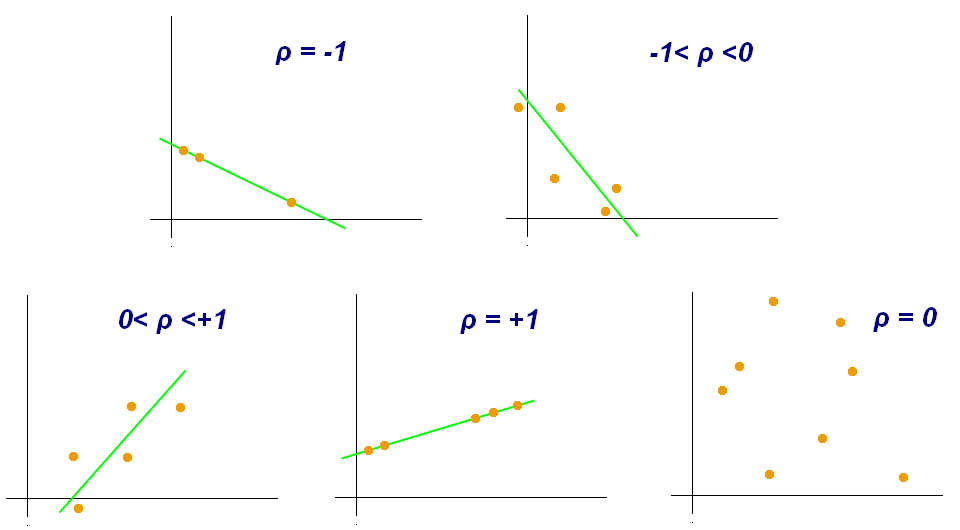
\includegraphics[width=0.6\linewidth]{PearsonCorrelation}
\end{center}
\[\rho=\frac{\Cov{X,Y}}{\sigma_X\sigma_Y}=\frac{\E{(X-\overline{X})(Y-\overline{Y})}}{\sqrt{\E{(X-\overline{X})^2}\E{(Y-\overline{Y})^2}}}\]
If instead of two random variables we are given a dataset $\mathcal{D}$, then the formula becomes:
\[\rho=\dfrac{\Sum_{i=1}^n\left(f(\vect{x}_i)-\overline{f}(\vect{x}_i)\right)\left(y_i-\overline{y}_i\right)}{\sqrt{\Sum_{i=1}^n\left(f(\vect{x}_i)-\overline{f}(\vect{x}_i)\right)^2\Sum_{i=1}^n\left(y_i-\overline{y}_i\right)^2}}\]
%
%
%
\section{Hold-out}
Since computing performance measure on the training set would be optimistically biased, we need to retain an independent set on which to compute performance. Moreover we'd like to have:
\begin{itemize}
  \item \textbf{Validation set}: when used to estimate performance of different algorithm settings, for instance when tuning the hyperparameters;
  \item \textbf{Test set}: when used to estimate the final performance of selected model.
\end{itemize}
One simple way to obtain this datasets is to divide the initial dataset into the three, usually with percentage as $40\%,30\%,30\%$ for training, validation and testing.
One problem with this procedure though is that the results depend on the specific test (and validation) set chosen, especially for small datasets. \newline
%
%
%
\section{$K$-Fold Cross Validation}
The hold-out method is used for big datasets, where we have a large amount of data and is less probable to obtain biased datasets. \newline
When such method is unusable, one could resolve to $k$-fold cross validation. The procedure is the following:
\begin{itemize}
  \item Split $\mathcal{D}$ into $k$ \textit{equal sized disjoint} subsets $\mathcal{D}_i$;
  \item For $i\in[1,k]$
    \begin{itemize}
      \item Train the predictor on $\mathcal{T}_i=\frac{\mathcal{D}}{\mathcal{D}_i}$
      \item Compute score $S$ on predictor $L(\mathcal{T}_i)$ on test set $\mathcal{D}_i$
        \[S_i=S_{\mathcal{D}_i}[L(\mathcal{T}_i)]\]
    \end{itemize}
  \item Return the average across folds:
    \[\overline{S}=\frac{1}{k}\Sum_{i=1}^kS_i\]
\end{itemize}
Basically is like saying that we do not trust the value that a hold-out procedure would return, but instead we prefer to have some kind of average. \newline
The idea is to split the dataset $\mathcal{D}$ into $k$ subsets, then to iterate through the various subsets keeping one for validation and the rest of the sub-datasets for training. Each time we'll compute the score and at the end average over all the scores. \newline
A part from the mean $\overline{S}$, one would like to compute also the variance of the mean:
\[\Var{\overline{S}}=\Var{\frac{S_1+\hdots+S_k}{k}}=\frac{1}{k^2}\Sum_{j=1}^k\Var{S_j}\]
The problem though is that we could compute $\Var{S_j}$ exactly only if all the training sets were independent, but this is not true since they have samples in common, so we have to approximate it with the unbiased variance across folds:
\[\Var{S_j}=\Var{S_h}\approx\frac{1}{k-1}\Sum_{i=1}^k\left(S_i-\overline{S}\right)^2\]
Giving:
\[\Var{\overline{S}}\approx\frac{1}{k^2}\Sum_{j=1}^k\left(\frac{1}{k-1}\Sum_{i=1}^k\left(S_i-\overline{S}\right)^2\right)=\frac{1}{k-1}\Sum_{i=1}^k\left(S_i-\overline{S}\right)^2\]
%
%
%
\section{Comparing Different Learning Algorithms}
Let's say we have two learning algorithms and we want to compare them. One possible way would just be to do cross validation and see which have the best statistics. The problem is that we want to be sure that the differences we see are \textit{statistically significant} and not due to some noisy evaluation. \newline
The most precise way to choose between two algorithms is to use \textbf{hypothesis testing} which allows to test the statistical significance of a hypothesis.\newline
In hypothesis testing we have a statement, called \textbf{null hypothesis} $H_0$, of which we want to prove the truthfulness, especially we want to provide \textit{prof} to reject the hypothesis. This is done with \textit{test statistic}: given a sample of $k$ realizations of random variables $X_1,\hdots,X_k$, a test statistic is a statistic $T=h(X_1,\hdots,X_k)$ whose value is used to decide whether to reject $H_0$ or not. Mind that not rejecting the hypothesis does not prove it to be true. \newline
\begin{definition}[Tail Probability]
  The probability that $T$ is at least as great (right tail) or at least as small (left tail) as the observed value $t$.
\end{definition}
\begin{definition}[p-Value]
  The probability of obtaining a value $T$ at least as extreme as the one observed $t$, in case $H_0$ is true.
\end{definition}
The p-value is also the value that allows to decide whether to accept or reject the null hypothesis. Given a threshold $\alpha$, if the p-value $p$ is higher than it, then the hypothesis may be accepted, otherwise it is rejected.  
\begin{definition}[Critical Region $\&$ Critical Values]
  The critical region is a set of values of $T$ for which we reject the null hypothesis. The critical values are the values on the boundary of the critical region. 
\end{definition}
We can define two possible errors:
\begin{itemize}
  \item Type I error: when we reject the null hypothesis when it's actually true;
  \item Type II error: when we accept the null hypothesis when it's actually false.
\end{itemize}
The \textbf{significance level} is the largest acceptable probability for committing a type I error. 
%
%
\subsection{T-Test}
The test statistic is given by the standardized (also called \textit{studentized}) mean:
\[T=\dfrac{\overline{X}-\mu_0}{\sqrt{\tilde{\Var{\overline{X}}}}}\]
where $\tilde{\Var{\overline{X}}}$ is the approximate variance and $\mu_0$ is the mean of the null distribution. \newline
Assuming all the samples come from an unknown Normal distribution, the test statistics has is a t-distribution which is a $k$-parametrized distribution with $k-1$ degree of freedom and with $k$ as the number of folds. The statistics is said to have a $t_{k-1}$ distribution under the null hypothesis. \newline
Given a significance level $\alpha$, the null hypothesis can be rejected if:
\[T\leq -t_{k-1,\frac{\alpha}{2}}, \qquad T\geq t_{k-1,\frac{\alpha}{2}}\]
%
\subsubsection{$t_{k-1}$-Distribution}
It's a bell-shaped distribution similar to the Normal one, though, it's wider and shorter: it reflects greater variance due to using $\tilde{\Var{\overline{X}}}$ instead of the true unknown variance of the distribution. \newline
$t_{k-1}$ tends to the standardized normal $z$ for $k\rightarrow\infty$, that is, the more number of folds we have, the more the t-distribution becomes similar to the Normal distribution.
\begin{center}
  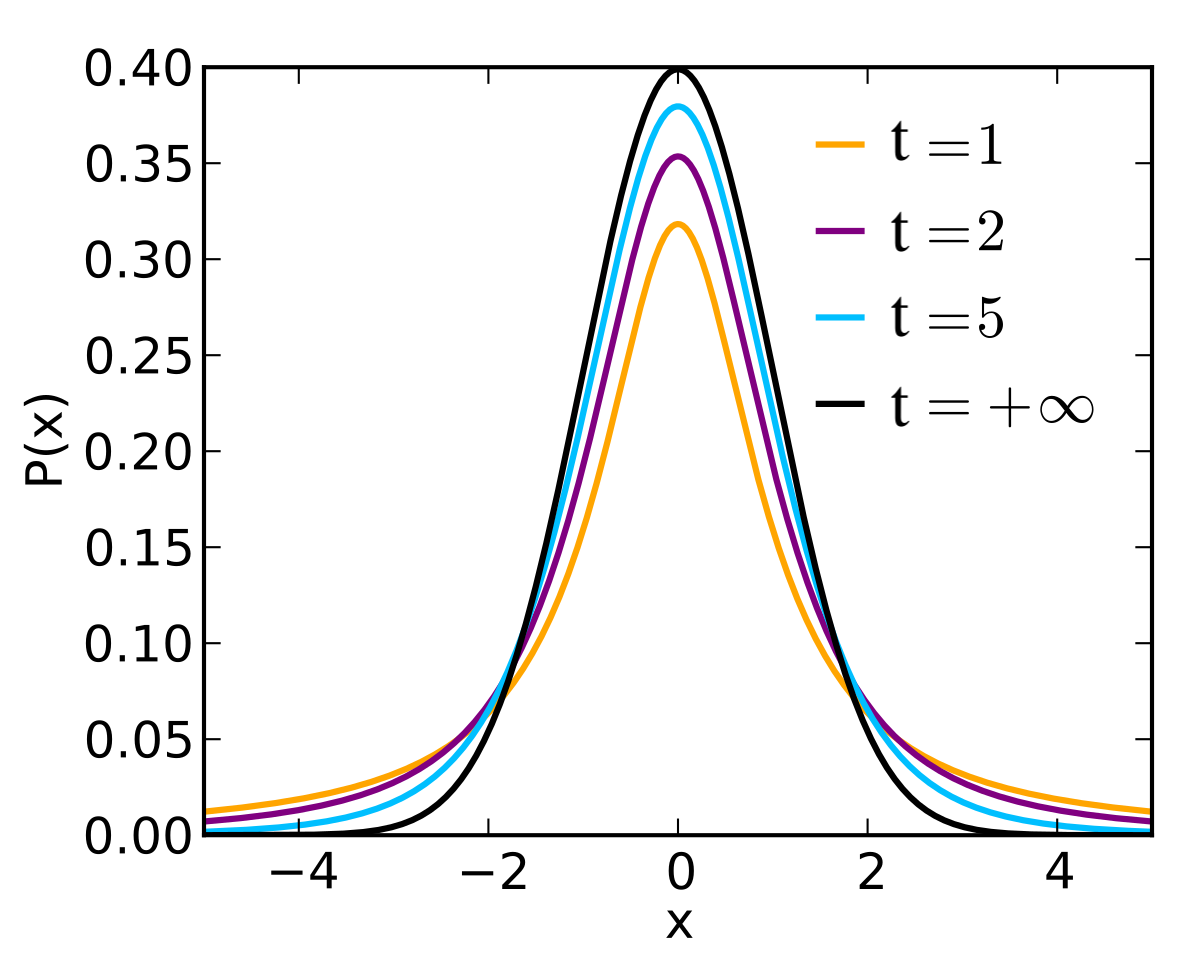
\includegraphics[width=0.6\linewidth]{TDistribution}
\end{center}
%
%
\subsection{How To}
Let's consider the case in which we have 2 algorithms $A$ and $B$ and we want to know which one works better. \newline
First of all, we shall run $k$-fold cross validation for algorithms $A$ and $B$. Then we'll compute the mean performance difference for the two algorithms:
\[\widehat{\delta}=\frac{1}{k}\Sum_{i=1}^k\delta_i=\frac{1}{k}\Sum_{i=1}^kS_{\mathcal{D}_i}[L_A(\mathcal{T}_i)]-S_{\mathcal{D}_i}[L_B(\mathcal{T}_i)]\]
where $S_{\mathcal{D_i}}[]$ is the score function chosen. \newline
Let's say that the null hypothesis is that the mean difference is 0. \newline
Let:
\[\sqrt{\tilde{\Var{\overline{\delta}}}}=\sqrt{\frac{1}{k(k-1)}\Sum_{i=1}^k)\delta_i-\overline{\delta})^2}\]
Given a significance level $\alpha$, i.e., the probability of resulting a type I error, we accept the null hypothesis if:
\[\frac{\overline{\delta}}{\sqrt{\tilde{\Var{\overline{\delta}}}}}\leq -t_{k-1,\frac{\alpha}{2}}\quad or\quad \frac{\overline{\delta}}{\sqrt{\tilde{\Var{\overline{\delta}}}}}\geq t_{k-1,\frac{\alpha}{2}}\]
Basically if the probability of type 1 error is on the tails of the distribution \newline
Note that the smaller $\alpha$, e.g. $5\%$, the smaller the probability of having an error. \newline
The T-test is called \textbf{pair test} because when we compute the two sample estimate, they come from the same fold, so we could compare the statistic on a certain fold. Moreover, it's also called \textbf{two-tailed test} because we cannot exclude at prior neither of the outcomes, i.e., if $A$ is better than $B$ or vice versa. Formally, no prior knowledge can tell the direction of the difference. If we knew that for $B$ is the worse case, hence it's not possible to do worse than that, then it would be a \textbf{one-tailed} test.
%
%
\subsection{T-Test Example}
We have two algorithms $A$ and $B$ and we want to know if they perform the same. Moreover, we have a dataset $\mathcal{D}$ and we are going to use $k$-fold cross validation with $k=10$. Let's say that the scores we obtain are:
\begin{center}
  \begin{tabular}{c|c|c}
    $\mathcal{D}_i$&$S_{\mathcal{D}_i}[L_A(\mathcal{T}_i)]$&$S_{\mathcal{D}_i}[L_A(\mathcal{T}_i)]$\\
  $\mathcal{D}_1$&0.81&0.80\\
  $\mathcal{D}_2$&0.82&0.77\\
  $\mathcal{D}_3$&0.84&0.70\\
  $\mathcal{D}_4$&0.78&0.83\\
  $\mathcal{D}_5$&0.85&0.80\\
  $\mathcal{D}_6$&0.86&0.78\\
  $\mathcal{D}_7$&0.82&0.75\\
  $\mathcal{D}_8$&0.83&0.80\\
  $\mathcal{D}_9$&0.82&0.78\\
  $\mathcal{D}_10$&0.81&0.77
  \end{tabular}
\end{center}
For each of them we can compute the difference between the scores of each fold $\delta$:
\[\widehat{\delta}=\frac{1}{k}\Sum_{i=1}^k\delta_i=\frac{1}{k}\Sum_{i=1}^kS_{\mathcal{D}_i}[L_A(\mathcal{T}_i)]-S_{\mathcal{D}_i}[L_B(\mathcal{T}_i)]\]
\begin{center}
  \begin{tabular}{c|c|c|c}
    $\mathcal{D}_i$&$S_{\mathcal{D}_i}[L_A(\mathcal{T}_i)]$&$S_{\mathcal{D}_i}[L_A(\mathcal{T}_i)]$&$\delta_i$\\
    $\mathcal{D}_1$&0.81&0.80&0.01\\
    $\mathcal{D}_2$&0.82&0.77&0.05\\
    $\mathcal{D}_3$&0.84&0.70&0.14\\
    $\mathcal{D}_4$&0.78&0.83&-0.05\\
    $\mathcal{D}_5$&0.85&0.80&0.05\\
    $\mathcal{D}_6$&0.86&0.78&0.08\\
    $\mathcal{D}_7$&0.82&0.75&0.07\\
    $\mathcal{D}_8$&0.83&0.80&0.03\\
    $\mathcal{D}_9$&0.82&0.78&0.04\\
    $\mathcal{D}_10$&0.81&0.77&0.04
  \end{tabular}
\end{center}
We the compute the average error difference:
\[\overline{\delta}=\frac{1}{10}\Sum_{i=1}^{10}\delta_i=0.046\]
We shall compute the unbiased estimate of the standard deviation:
\[\sqrt{\tilde{\Var{\overline{\delta}}}}=\sqrt{\frac{1}{10\times 9}\Sum_{i=1}^{10}\left(\delta_i-\overline{\delta}\right)^2}=0.0154344\]
The standardized mean error difference is:
\[\frac{\overline{\delta}}{\sqrt{\tilde{\Var{\overline{\delta}}}}}=\frac{0.046}{0.0154344}=2.98\]
Since $\alpha=5\%$ is a good threshold, then we have:
\[t_{k-1,\frac{\alpha}{2}}=t_{9,0.025}=2.262<2.98\]
Since the value is nor smaller than -2.98, nor greater than 2.98, then the null hypothesis is rejected, the classifiers are actually different. 
\begin{center}
  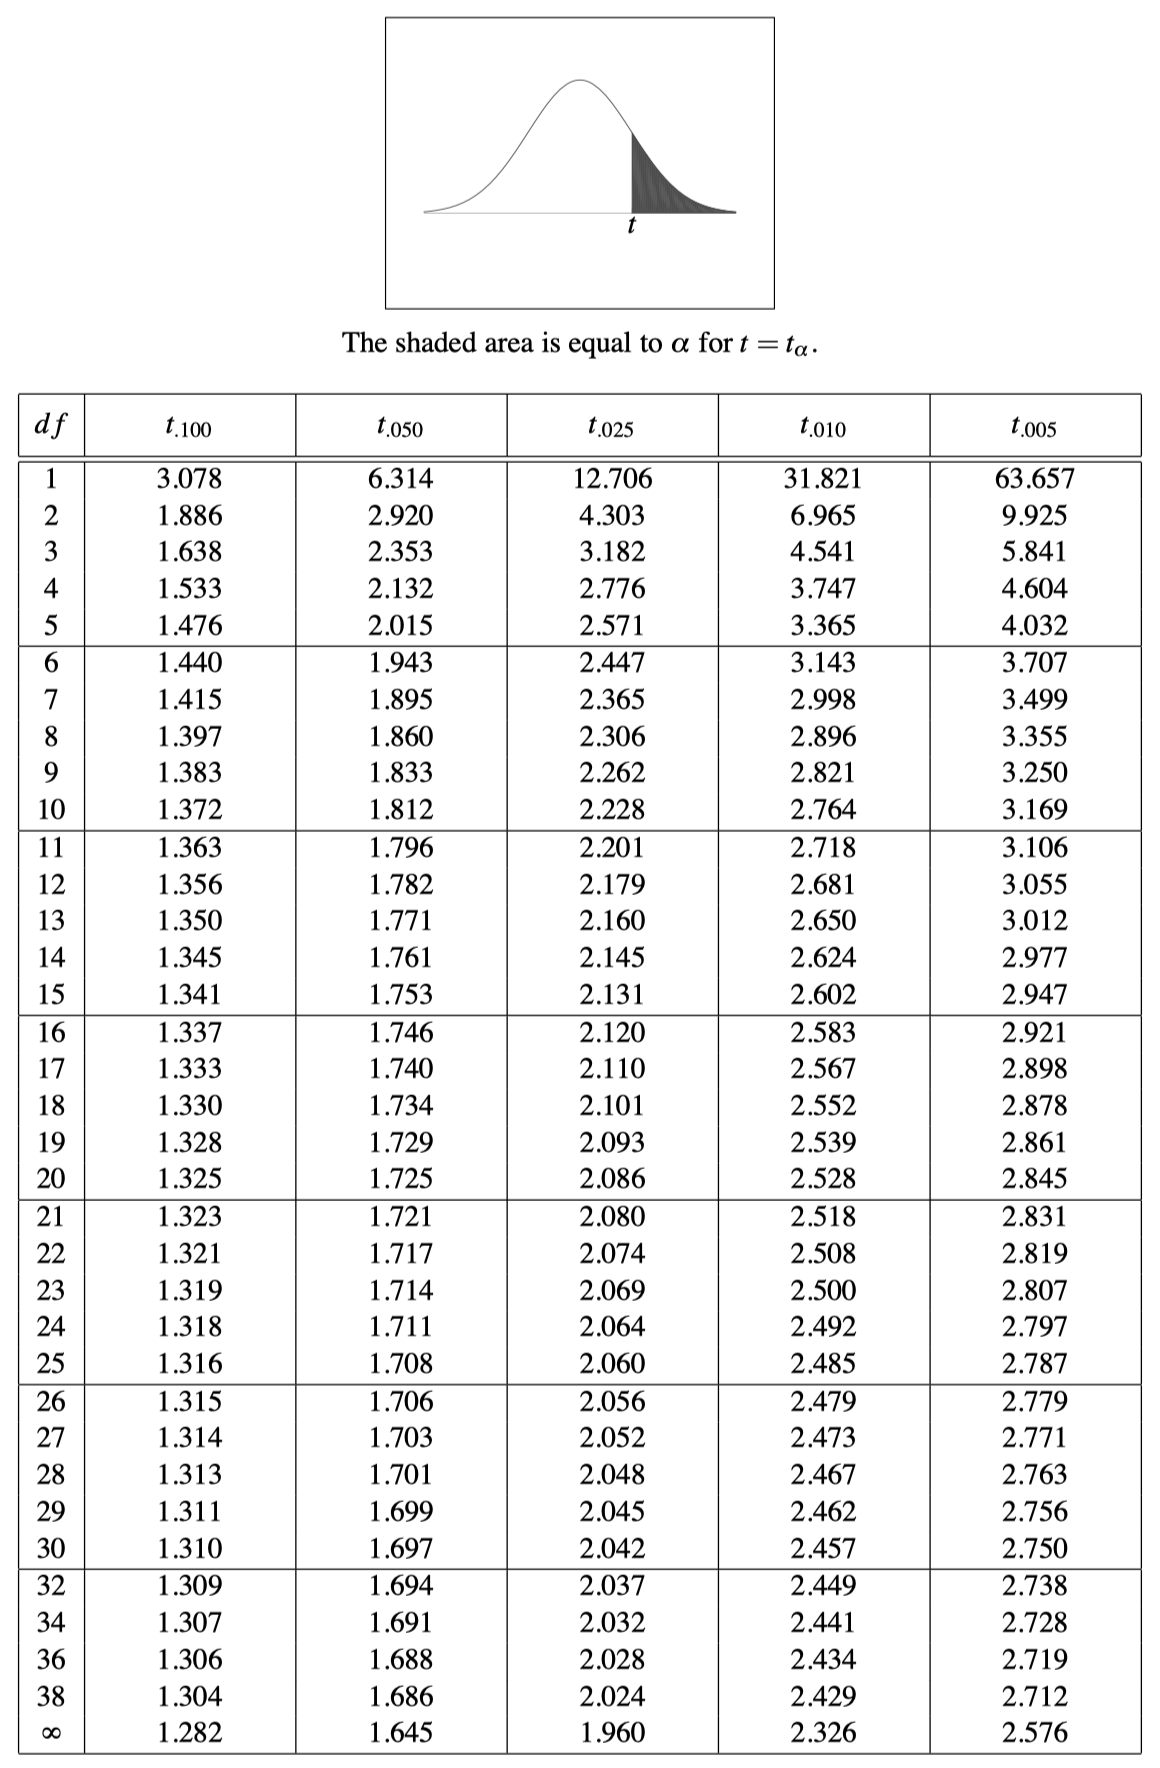
\includegraphics[width=0.7\linewidth]{tDistributionTable}
\end{center}





